\documentclass[aspectratio=169]{beamer}

% -------------------------
% 1.  PACKAGES & THEME
% -------------------------
\usepackage[english]{babel}
\usepackage{fontawesome5}
\usepackage{tikz}
\usetikzlibrary{positioning,calc,shapes.geometric,backgrounds,patterns}
\usepackage{helvet}
\renewcommand{\familydefault}{\sfdefault}
\usepackage{graphicx}
\usepackage{hyperref}
\usepackage{booktabs}
\usepackage{pgf-pie}
\usepackage{xcolor}

% Theme & colors - WRAPSYNTH DARK MODE: ORANGE / GREY / BLACK
\usetheme{metropolis}

% Primary brand colors
\definecolor{primary}{HTML}{FF6B1A}        % WrapSynth orange (main accent)
\definecolor{secondary}{HTML}{4A4A4A}      % Medium grey (borders, secondary elements)
\definecolor{accent}{HTML}{8C8C8C}         % Lighter grey (captions, subtle UI)

% Background colors - dark mode
\definecolor{darkbg}{HTML}{0D0D0D}         % Near-black (main background)
\definecolor{midbg}{HTML}{1A1A1A}          % Dark grey (panels)
\definecolor{lightbg}{HTML}{2A2A2A}        % Slightly lighter dark grey (cards)

% Text and UI colors - high contrast on dark
\definecolor{textprimary}{HTML}{F5F5F5}    % Near-white (primary text)
\definecolor{textsecondary}{HTML}{B0B0B0}  % Light grey (secondary text)
\definecolor{highlight}{HTML}{FF6B1A}      % Orange for special emphasis

% Semantic colors
\definecolor{success}{HTML}{4CAF50}        % Green (positive/success)
\definecolor{warning}{HTML}{FF6B1A}        % Orange (warning/important)
\definecolor{info}{HTML}{8C8C8C}           % Grey (info/neutral)
\definecolor{danger}{HTML}{E53935}         % Red (negative/centralized)

\setbeamercolor{background canvas}{bg=darkbg}
\setbeamercolor{normal text}{fg=textprimary}
\setbeamercolor{alerted text}{fg=primary}
\setbeamercolor{example text}{fg=secondary}
\setbeamercolor{frametitle}{fg=textprimary,bg=darkbg}
\setbeamercolor{title}{fg=textprimary}

\setbeamerfont{title}{size=\Huge,series=\bfseries}
\setbeamerfont{subtitle}{size=\Large}
\setbeamerfont{author}{size=\normalsize}
\setbeamerfont{date}{size=\small}
\setbeamerfont{frametitle}{size=\Large,series=\bfseries}

% No nav symbols, clean footer with slide numbers
\setbeamertemplate{navigation symbols}{}
\setbeamertemplate{footline}{%
  \hfill%
  \usebeamerfont{page number in head/foot}%
  \color{textsecondary}\insertframenumber\,/\,\inserttotalframenumber\kern1em\vskip2pt%
}

% Custom itemize bullets
\setbeamertemplate{itemize items}[circle]
\setbeamercolor{itemize item}{fg=primary}
\setbeamercolor{itemize subitem}{fg=secondary}

% -------------------------
% 2.  TITLE SLIDE
% -------------------------
\title{WrapSynth}

\begin{document}

% -------------------------------------------------
\begin{frame}[plain]
  \begin{tikzpicture}[remember picture,overlay]
    % Dark background
    \fill[darkbg] (current page.south west) rectangle (current page.north east);
    
    % Subtle orange gradient overlay
    \fill[primary,opacity=0.06] (current page.south west) -- 
          (current page.north west) -- 
          ([yshift=-3cm]current page.north east) -- 
          ([yshift=2cm]current page.south east) -- cycle;
    
    % Subtle dot pattern
    \foreach \x in {0,1,2,...,20} {
      \foreach \y in {0,1,2,...,12} {
        \fill[secondary,opacity=0.03] ([shift={(0.8*\x cm, 0.8*\y cm)}]current page.south west) circle (0.5pt);
      }
    }
    
    % Main title: offset drop shadow + two-tone text
    \node[anchor=south] at ($(current page.center)+(0.09,0.36)$){
      \fontsize{72}{80}\selectfont\color{primary!45!darkbg}\textbf{WrapSynth}
    };
    \node[anchor=south] at ($(current page.center)+(0,0.45)$){
      \fontsize{72}{80}\selectfont\textbf{\color{textprimary}Wrap\color{primary}Synth}
    };
    % Subtitle
    \node[anchor=north,align=center] at ($(current page.center)+(0,0.25)$){
      {\fontsize{28}{36}\selectfont\color{primary}\textbf{Trustless XMR Settlement}}\\[0.4em]
      {\fontsize{20}{28}\selectfont\color{textsecondary}Disrupting Centralized Monero Bridges}
    };
    
    % Orange accent lines
    \fill[primary,opacity=0.8] (current page.south west) -- ++(3,0) -- ++(0,0.12) -- ++(-3,0) -- cycle;
    \fill[primary,opacity=0.8] (current page.north east) -- ++(-3,0) -- ++(0,-0.12) -- ++(3,0) -- cycle;
    
  \end{tikzpicture}
\end{frame}

% -------------------------------------------------
\begin{frame}[t]{\color{textsecondary}\textbf{The Competition: Centralized Bridges with Proven Demand}}

  \vspace{0.3em}
  
  \begin{tikzpicture}
    % Three competitor boxes side by side
    
    % Wagyu (Hyperliquid)
    \fill[lightbg,rounded corners=12pt] (-7.2,-3.5) rectangle (-2.5,3.2);
    \draw[danger,line width=1.5pt,rounded corners=12pt] (-7.2,-3.5) rectangle (-2.5,3.2);
    \node[text=danger,font=\large\bfseries] at (-4.85,2.7) {Wagyu};
    \node[text=textsecondary,font=\small] at (-4.85,2.2) {Hyperliquid};
    \node[text=primary,font=\Large\bfseries] at (-4.85,1.3) {\$700M};
    \node[text=textsecondary,font=\scriptsize,align=center] at (-4.85,0.8) {cumulative volume};
    \node[text=textprimary,font=\scriptsize,align=center,text width=4cm] at (-4.85,-0.2) {Centralized bridge\\Anonymous operator\\No proof-of-reserves};
    \node[text=danger,font=\scriptsize,align=center] at (-4.85,-2.0) {\faTimesCircle\ \ Allegedly went dark};
    \node[text=textsecondary,font=\scriptsize,align=center] at (-4.85,-2.8) {2\% fee on XMR routes};
    
    % WXMR (Solana)
    \fill[lightbg,rounded corners=12pt] (-2.2,-3.5) rectangle (2.5,3.2);
    \draw[danger,line width=1.5pt,rounded corners=12pt] (-2.2,-3.5) rectangle (2.5,3.2);
    \node[text=danger,font=\large\bfseries] at (0.15,2.7) {WXMR};
    \node[text=textsecondary,font=\small] at (0.15,2.2) {Solana / Jupiter};
    \node[text=primary,font=\Large\bfseries] at (0.15,1.3) {\$12M/day};
    \node[text=textsecondary,font=\scriptsize,align=center] at (0.15,0.8) {trading volume};
    \node[text=textprimary,font=\scriptsize,align=center,text width=4cm] at (0.15,-0.2) {Centralized wrap\\Unverifiable reserves\\26.3K holders};
    \node[text=textsecondary,font=\scriptsize,align=center] at (0.15,-2.0) {\faIcon{exchange-alt}\ \ Trust the issuer};
    \node[text=textsecondary,font=\scriptsize,align=center] at (0.15,-2.8) {\$662K liquidity};
    
    % Instant Swaps
    \fill[lightbg,rounded corners=12pt] (2.8,-3.5) rectangle (7.5,3.2);
    \draw[danger,line width=1.5pt,rounded corners=12pt] (2.8,-3.5) rectangle (7.5,3.2);
    \node[text=danger,font=\large\bfseries] at (5.15,2.7) {Instant Swaps};
    \node[text=textsecondary,font=\small] at (5.15,2.2) {ChangeNOW, SideShift, etc.};
    \node[text=primary,font=\Large\bfseries] at (5.15,1.3) {1--4\%};
    \node[text=textsecondary,font=\scriptsize,align=center] at (5.15,0.8) {effective all-in cost};
    \node[text=textprimary,font=\scriptsize,align=center,text width=4cm] at (5.15,-0.2) {Principal inventory model\\No orderbook\\Unbenchmarkable rates};
    \node[text=textsecondary,font=\scriptsize,align=center] at (5.15,-2.0) {\faUserShield\ \ Custodial risk};
    \node[text=textsecondary,font=\scriptsize,align=center] at (5.15,-2.8) {\$1 flat fee on small swaps};
    
  \end{tikzpicture}

\end{frame}

% -------------------------------------------------
\begin{frame}[t]{\color{textsecondary}\textbf{Why Now: The Market is Ready}}

  \centering
  
  \begin{tikzpicture}
    % Six "why now" factors in 2 rows of 3
    
    % Row 1
    \begin{scope}[shift={(-4.5,1.8)}]
      \fill[lightbg,rounded corners=12pt] (-2.3,-1.2) rectangle (2.3,1.2);
      \draw[primary,line width=0.8pt,rounded corners=12pt] (-2.3,-1.2) rectangle (2.3,1.2);
      \node[text=primary,font=\Large] at (0,0.55) {\faChartLine};
      \node[text=textprimary,font=\small\bfseries,align=center,text width=4cm] at (0,-0.35) {\$700M+ proven demand\\for synthetic XMR};
    \end{scope}
    
    \begin{scope}[shift={(0,1.8)}]
      \fill[lightbg,rounded corners=12pt] (-2.3,-1.2) rectangle (2.3,1.2);
      \draw[primary,line width=0.8pt,rounded corners=12pt] (-2.3,-1.2) rectangle (2.3,1.2);
      \node[text=primary,font=\Large] at (0,0.55) {\faBan};
      \node[text=textprimary,font=\small\bfseries,align=center,text width=4cm] at (0,-0.35) {CEX delistings\\accelerating};
    \end{scope}
    
    \begin{scope}[shift={(4.5,1.8)}]
      \fill[lightbg,rounded corners=12pt] (-2.3,-1.2) rectangle (2.3,1.2);
      \draw[primary,line width=0.8pt,rounded corners=12pt] (-2.3,-1.2) rectangle (2.3,1.2);
      \node[text=primary,font=\Large] at (0,0.55) {\faRocket};
      \node[text=textprimary,font=\small\bfseries,align=center,text width=4cm] at (0,-0.35) {XMR to \$4000 on Jupiter\\speculative demand proven};
    \end{scope}
    
    % Row 2
    \begin{scope}[shift={(-4.5,-1.8)}]
      \fill[lightbg,rounded corners=12pt] (-2.3,-1.2) rectangle (2.3,1.2);
      \draw[primary,line width=0.8pt,rounded corners=12pt] (-2.3,-1.2) rectangle (2.3,1.2);
      \node[text=primary,font=\Large] at (0,0.55) {\faNetworkWired};
      \node[text=textprimary,font=\small\bfseries,align=center,text width=4cm] at (0,-0.35) {HyperEVM + Solana\\deployment venues live};
    \end{scope}
    
    \begin{scope}[shift={(0,-1.8)}]
      \fill[lightbg,rounded corners=12pt] (-2.3,-1.2) rectangle (2.3,1.2);
      \draw[primary,line width=0.8pt,rounded corners=12pt] (-2.3,-1.2) rectangle (2.3,1.2);
      \node[text=primary,font=\Large] at (0,0.55) {\faIcon{shield-alt}};
      \node[text=textprimary,font=\small\bfseries,align=center,text width=4cm] at (0,-0.35) {Atomic swap tech\\proven and audited};
    \end{scope}
    
    \begin{scope}[shift={(4.5,-1.8)}]
      \fill[lightbg,rounded corners=12pt] (-2.3,-1.2) rectangle (2.3,1.2);
      \draw[primary,line width=0.8pt,rounded corners=12pt] (-2.3,-1.2) rectangle (2.3,1.2);
      \node[text=primary,font=\Large] at (0,0.55) {\faTrophy};
      \node[text=textprimary,font=\small\bfseries,align=center,text width=4cm] at (0,-0.35) {Colosseum hackathon\\+ Hyperliquid track};
    \end{scope}
  \end{tikzpicture}
\end{frame}

% -------------------------------------------------
\begin{frame}{\color{textsecondary}\textbf{WrapSynth: Trustless Settlement Architecture}}

  \centering

  \begin{tikzpicture}
    % Three pillars - Atomic Swaps, LP Vaults, Multi-chain
    
    % Atomic Swaps
    \fill[lightbg,rounded corners=12pt] (-6.8,0) rectangle (-2.6,4.2);
    \draw[primary,line width=1.5pt,rounded corners=12pt] (-6.8,0) rectangle (-2.6,4.2);
    \node[text=primary,font=\Huge] at (-4.7,3) {\faRandom};
    \node[text=textprimary,font=\large\bfseries,align=center] at (-4.7,1.8) {Ed25519\\Atomic Swaps};
    \node[text=textsecondary,font=\scriptsize,align=center,text width=3.5cm] at (-4.7,0.6) {Peer-to-peer settlement\\On-chain secret verification\\No trusted operator};
    
    % Overcollateralized LP Vaults
    \fill[lightbg,rounded corners=12pt] (-2.1,0) rectangle (2.1,4.2);
    \draw[primary,line width=1.5pt,rounded corners=12pt] (-2.1,0) rectangle (2.1,4.2);
    \node[text=primary,font=\Huge] at (0,3) {\faLock};
    \node[text=textprimary,font=\large\bfseries,align=center] at (0,1.8) {Overcollateralized\\LP Vaults};
    \node[text=textsecondary,font=\scriptsize,align=center,text width=3.5cm] at (0,0.6) {USDe collateral (HyperEVM)\\JitoSOL (Solana)\\On-chain slashing};
    
    % Multi-chain
    \fill[lightbg,rounded corners=12pt] (2.6,0) rectangle (6.8,4.2);
    \draw[primary,line width=1.5pt,rounded corners=12pt] (2.6,0) rectangle (6.8,4.2);
    \node[text=primary,font=\Huge] at (4.7,3) {\faLink};
    \node[text=textprimary,font=\large\bfseries,align=center] at (4.7,1.8) {Multi-Chain\\Wrapped Tokens};
    \node[text=textsecondary,font=\scriptsize,align=center,text width=3.5cm] at (4.7,0.6) {HyperEVM (ERC-20 + HIP-1)\\Solana (SPL)\\Robinhood Chain (Q4)};
  \end{tikzpicture}
  
\end{frame}

% -------------------------------------------------
\begin{frame}[t]{\color{textsecondary}\textbf{Live on HyperEVM}}

  \centering
  \vspace{0.5em}
  
  \begin{tikzpicture}
    % Deployment proof box
    \fill[lightbg,rounded corners=15pt] (-7,-3.5) rectangle (7,3.5);
    \draw[primary,line width=1pt,rounded corners=15pt] (-7,-3.5) rectangle (7,3.5);
    
    % Header
    \node[text=primary,font=\Large\bfseries] at (0,2.8) {\faCheckCircle\ \ Deployed and Verified};
    
    % Three columns of proof points
    \node[text=textprimary,font=\small\bfseries,align=center] at (-4,1.8) {Contracts};
    \node[text=textsecondary,font=\scriptsize,align=center,text width=3.5cm] at (-4,0.8) {wsXmrHub (Diamond)\\VaultFacet\\MintFacet\\BurnFacet\\LiquidationFacet\\YieldFacet\\RedStoneOracleFacet};
    
    \node[text=textprimary,font=\small\bfseries,align=center] at (0,1.8) {Collateral};
    \node[text=textsecondary,font=\scriptsize,align=center,text width=3.5cm] at (0,0.8) {USDe via HyperLend\\10\% raw-USDe buffer\\150/180/120 ratios\\On-chain slashing\\Trustless settlement};
    
    \node[text=textprimary,font=\small\bfseries,align=center] at (4,1.8) {Security};
    \node[text=textsecondary,font=\scriptsize,align=center,text width=3.5cm] at (4,0.8) {lockHub() executed\\lockDeployer() executed\\EIP-1153 delegate context\\633-line invariant suite\\Two security reviews};
    
    % Bottom emphasis
    \node[text=primary,font=\normalsize\bfseries,align=center] at (0,-1.8) {Same settlement model, now on the chain where XMR demand actually trades};
    \node[text=textsecondary,font=\small,align=center] at (0,-2.5) {Demo: wrapsynth.com};
    
  \end{tikzpicture}
\end{frame}

% -------------------------------------------------
\begin{frame}[t]{\color{textsecondary}\textbf{Competitive Advantages}}

  \centering

  \begin{tikzpicture}
    % Four advantages stacked
    
    % Trustless vs Centralized
    \fill[lightbg,rounded corners=15pt] (-7,2.2) rectangle (7,3.4);
    \draw[primary,line width=0.5pt,rounded corners=15pt] (-7,2.2) rectangle (7,3.4);
    \node[text=primary,font=\Large] at (-6,2.8) {\faIcon{shield-alt}};
    \node[text=textprimary,font=\large\bfseries,align=left,anchor=west] at (-5.2,2.8) {Trustless atomic swaps vs ``trust the operator''};
    
    % On-chain solvency
    \fill[lightbg,rounded corners=15pt] (-7,0.9) rectangle (7,2.0);
    \draw[primary,line width=0.5pt,rounded corners=15pt] (-7,0.9) rectangle (7,2.0);
    \node[text=primary,font=\Large] at (-6,1.45) {\faSearchDollar};
    \node[text=textprimary,font=\large\bfseries,align=left,anchor=west] at (-5.2,1.45) {On-chain proof of solvency vs unverifiable XMR reserves};
    
    % DeFi composability
    \fill[lightbg,rounded corners=15pt] (-7,-0.4) rectangle (7,0.7);
    \draw[primary,line width=0.5pt,rounded corners=15pt] (-7,-0.4) rectangle (7,0.7);
    \node[text=primary,font=\Large] at (-6,0.15) {\faCubes};
    \node[text=textprimary,font=\large\bfseries,align=left,anchor=west] at (-5.2,0.15) {Full ERC-20 composability vs dead-end HyperCore-only assets};
    
    % Multi-chain
    \fill[lightbg,rounded corners=15pt] (-7,-1.7) rectangle (7,-0.6);
    \draw[primary,line width=0.5pt,rounded corners=15pt] (-7,-1.7) rectangle (7,-0.6);
    \node[text=primary,font=\Large] at (-6,-1.15) {\faNetworkWired};
    \node[text=textprimary,font=\large\bfseries,align=left,anchor=west] at (-5.2,-1.15) {Multi-chain deployment vs single-venue lock-in};
    
  \end{tikzpicture}
\end{frame}

% -------------------------------------------------
\begin{frame}[t]{\color{textsecondary}\textbf{Real Revenue: Market Making + Protocol Fees}}

  \centering
  \vspace{0.5em}
  
  \begin{tikzpicture}
    % Revenue streams in 3 columns
    
    % Market Making (the proof)
    \fill[lightbg,rounded corners=12pt] (-7,-3) rectangle (-2.5,3.2);
    \draw[primary,line width=1.5pt,rounded corners=12pt] (-7,-3) rectangle (-2.5,3.2);
    \node[text=primary,font=\Large] at (-4.75,2.6) {\faChartBar};
    \node[text=textprimary,font=\normalsize\bfseries,align=center] at (-4.75,1.8) {Market Making};
    \node[text=primary,font=\Large\bfseries,align=center] at (-4.75,0.9) {5-figure profit};
    \node[text=textsecondary,font=\scriptsize,align=center] at (-4.75,0.3) {Q3 2026};
    \node[text=textsecondary,font=\scriptsize,align=center,text width=4cm] at (-4.75,-0.8) {Arbitraging XMR between\\Wagyu, WXMR, and\\instant swap services};
    \node[text=primary,font=\scriptsize\bfseries,align=center] at (-4.75,-2.1) {Bulk from XMR \$4000 run};
    \node[text=textsecondary,font=\scriptsize,align=center] at (-4.75,-2.6) {on Jupiter};
    
    % Protocol Fees
    \fill[lightbg,rounded corners=12pt] (-2.2,-3) rectangle (2.5,3.2);
    \draw[secondary,line width=1.5pt,rounded corners=12pt] (-2.2,-3) rectangle (2.5,3.2);
    \node[text=primary,font=\Large] at (0.15,2.6) {\faCoins};
    \node[text=textprimary,font=\normalsize\bfseries,align=center] at (0.15,1.8) {Protocol Fees};
    \node[text=textsecondary,font=\scriptsize,align=center,text width=4cm] at (0.15,0.8) {Mint/burn fees\\on atomic swaps};
    \node[text=textsecondary,font=\scriptsize,align=center,text width=4cm] at (0.15,-0.2) {LP collateral yield\\(USDe supply APY)};
    \node[text=textsecondary,font=\scriptsize,align=center,text width=4cm] at (0.15,-1.2) {HIP-3 perp fees\\(up to 50\% share)};
    \node[text=textsecondary,font=\scriptsize,align=center,text width=4cm] at (0.15,-2.2) {Spread capture\\between venues};
    
    % The Edge
    \fill[lightbg,rounded corners=12pt] (2.8,-3) rectangle (7.5,3.2);
    \draw[secondary,line width=1.5pt,rounded corners=12pt] (2.8,-3) rectangle (7.5,3.2);
    \node[text=primary,font=\Large] at (5.15,2.6) {\faIcon{exchange-alt}};
    \node[text=textprimary,font=\normalsize\bfseries,align=center] at (5.15,1.8) {The Spread Edge};
    \node[text=textsecondary,font=\scriptsize,align=center,text width=4cm] at (5.15,0.9) {Solana XMR operator\\partnership:};
    \node[text=success,font=\scriptsize\bfseries,align=center] at (5.15,0.2) {0\% onramp fee};
    \node[text=success,font=\scriptsize\bfseries,align=center] at (5.15,-0.3) {10bps offramp};
    \node[text=textsecondary,font=\scriptsize,align=center,text width=4cm] at (5.15,-1.1) {vs Wagyu's 2\%\\vs instant swaps' \$1};
    \node[text=primary,font=\scriptsize\bfseries,align=center] at (5.15,-2.2) {We fill the gap};
    
  \end{tikzpicture}
\end{frame}

% -------------------------------------------------
\begin{frame}{\color{textsecondary}\textbf{Live Web App}}
  
  % Two column layout
  \begin{columns}[c]
    % Left column for text
    \begin{column}{0.45\textwidth}
      \centering
      
      {\LARGE\color{primary}\textbf{WRAPSYNTH}}
      
      \vspace{0.5em}
      
      {\normalsize\color{textsecondary}Live demo:}
      
      {\normalsize\color{primary}\textbf{wrapsynth.com}}
      
    \end{column}
    
    % Right column for image
    \begin{column}{0.55\textwidth}
      \centering
      \includegraphics[height=0.75\textheight,width=\textwidth,keepaspectratio]{ui.png}
    \end{column}
  \end{columns}
  
\end{frame}

% -------------------------------------------------
\begin{frame}[t]{\color{textsecondary}\textbf{The Market is Immense}}

  \centering
  \vspace{2em}
  
  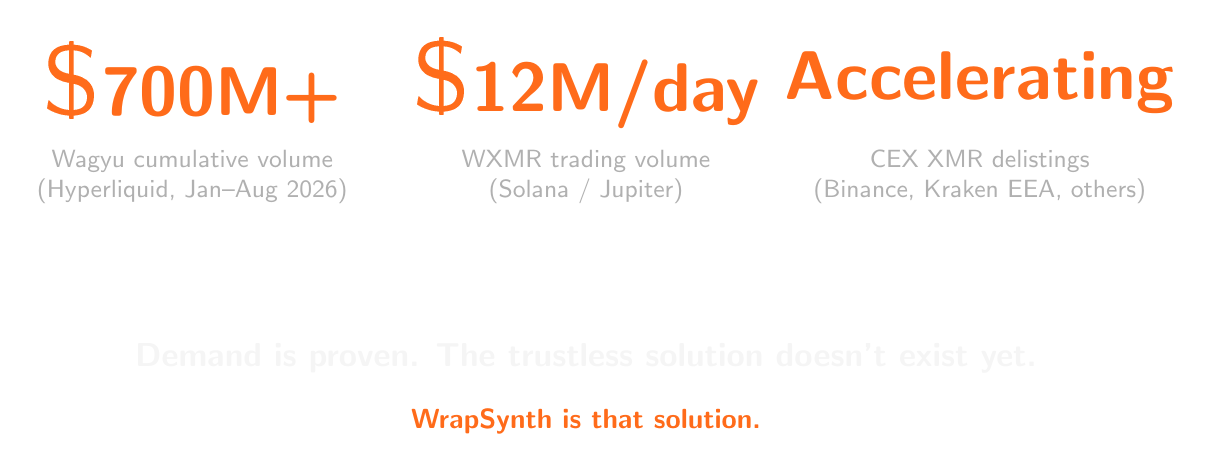
\begin{tikzpicture}
    % Key market figures
    
    % Wagyu volume
    \node[text=primary,font=\fontsize{42}{50}\selectfont\bfseries] at (-5,2) {\$700M+};
    \node[text=textsecondary,font=\small,align=center] at (-5,0.8) {Wagyu cumulative volume\\(Hyperliquid, Jan--Aug 2026)};
    
    % WXMR daily
    \node[text=primary,font=\fontsize{42}{50}\selectfont\bfseries] at (0,2) {\$12M/day};
    \node[text=textsecondary,font=\small,align=center] at (0,0.8) {WXMR trading volume\\(Solana / Jupiter)};
    
    % Delistings
    \node[text=primary,font=\fontsize{42}{50}\selectfont\bfseries] at (5,2) {Accelerating};
    \node[text=textsecondary,font=\small,align=center] at (5,0.8) {CEX XMR delistings\\(Binance, Kraken EEA, others)};
    
    % Bottom line
    \node[text=textprimary,font=\large\bfseries,align=center] at (0,-1.5) {Demand is proven. The trustless solution doesn't exist yet.};
    \node[text=primary,font=\normalsize\bfseries,align=center] at (0,-2.3) {WrapSynth is that solution.};
  \end{tikzpicture}
\end{frame}

% -------------------------------------------------
\begin{frame}[t]{\color{textsecondary}\textbf{Roadmap}}

  \centering
  \vspace{1em}
  
  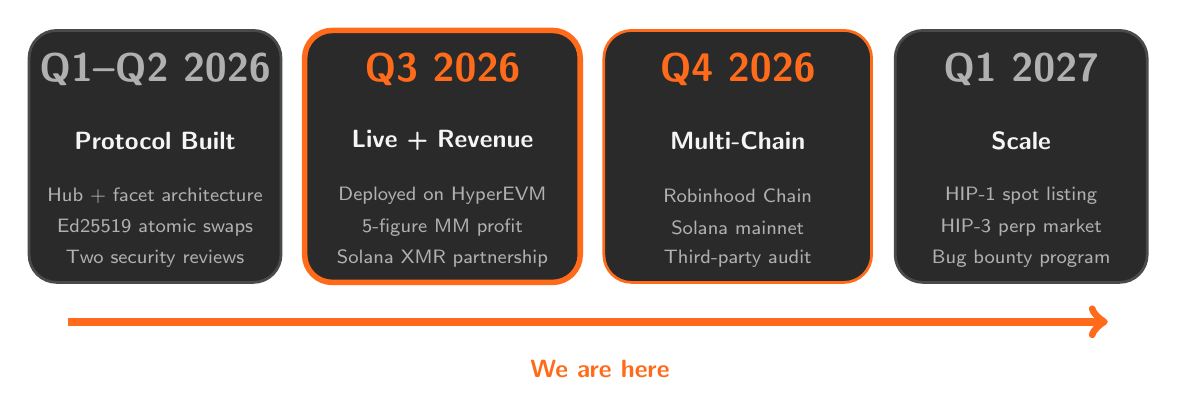
\begin{tikzpicture}
    % Q1-Q2 2026
    \fill[lightbg,rounded corners=10pt] (-7.5,2.8) rectangle (-4.3,6.0);
    \draw[secondary,line width=1pt,rounded corners=10pt] (-7.5,2.8) rectangle (-4.3,6.0);
    \node[text=textsecondary,font=\Large\bfseries] at (-5.9,5.5) {Q1--Q2 2026};
    \node[text=textprimary,font=\small\bfseries,align=center] at (-5.9,4.6) {Protocol Built};
    \node[text=textsecondary,font=\scriptsize,align=center] at (-5.9,3.9) {Hub + facet architecture};
    \node[text=textsecondary,font=\scriptsize,align=center] at (-5.9,3.5) {Ed25519 atomic swaps};
    \node[text=textsecondary,font=\scriptsize,align=center] at (-5.9,3.1) {Two security reviews};
    
    % Q3 2026 (current - highlighted)
    \fill[lightbg,rounded corners=10pt] (-4,2.8) rectangle (-0.5,6.0);
    \draw[primary,line width=2pt,rounded corners=10pt] (-4,2.8) rectangle (-0.5,6.0);
    \node[text=primary,font=\Large\bfseries] at (-2.25,5.5) {Q3 2026};
    \node[text=textprimary,font=\small\bfseries,align=center] at (-2.25,4.6) {Live + Revenue};
    \node[text=textsecondary,font=\scriptsize,align=center] at (-2.25,3.9) {Deployed on HyperEVM};
    \node[text=textsecondary,font=\scriptsize,align=center] at (-2.25,3.5) {5-figure MM profit};
    \node[text=textsecondary,font=\scriptsize,align=center] at (-2.25,3.1) {Solana XMR partnership};
    
    % Q4 2026
    \fill[lightbg,rounded corners=10pt] (-0.2,2.8) rectangle (3.2,6.0);
    \draw[primary,line width=1pt,rounded corners=10pt] (-0.2,2.8) rectangle (3.2,6.0);
    \node[text=primary,font=\Large\bfseries] at (1.5,5.5) {Q4 2026};
    \node[text=textprimary,font=\small\bfseries,align=center] at (1.5,4.6) {Multi-Chain};
    \node[text=textsecondary,font=\scriptsize,align=center] at (1.5,3.9) {Robinhood Chain};
    \node[text=textsecondary,font=\scriptsize,align=center] at (1.5,3.5) {Solana mainnet};
    \node[text=textsecondary,font=\scriptsize,align=center] at (1.5,3.1) {Third-party audit};
    
    % Q1 2027
    \fill[lightbg,rounded corners=10pt] (3.5,2.8) rectangle (6.7,6.0);
    \draw[secondary,line width=1pt,rounded corners=10pt] (3.5,2.8) rectangle (6.7,6.0);
    \node[text=textsecondary,font=\Large\bfseries] at (5.1,5.5) {Q1 2027};
    \node[text=textprimary,font=\small\bfseries,align=center] at (5.1,4.6) {Scale};
    \node[text=textsecondary,font=\scriptsize,align=center] at (5.1,3.9) {HIP-1 spot listing};
    \node[text=textsecondary,font=\scriptsize,align=center] at (5.1,3.5) {HIP-3 perp market};
    \node[text=textsecondary,font=\scriptsize,align=center] at (5.1,3.1) {Bug bounty program};
    
    % Timeline arrow
    \draw[->,line width=3pt,primary] (-7,2.3) -- (6.2,2.3);
    \node[text=primary,font=\small\bfseries] at (-0.25,1.7) {We are here};
    
  \end{tikzpicture}
\end{frame}

% -------------------------------------------------
\begin{frame}[t]{\color{textsecondary}\textbf{Cypherpunk Founders}}
  
  \centering
  \vspace{-1em}
  
  \begin{tikzpicture}
    % Container bubble
    \fill[lightbg,rounded corners=20pt] (-7,-2.5) rectangle (7,4.0);
    \draw[primary,line width=1pt,rounded corners=20pt] (-7,-2.5) rectangle (7,4.0);
    
    % MADS - Left founder
    \fill[midbg,rounded corners=8pt] (-6,-0.5) rectangle (-1.5,3.6);
    \node[text=textprimary,font=\bfseries,align=center] at (-3.75,3.3) {Mads Christensen};
    % Image with frame
    \begin{scope}
      \clip[rounded corners=4pt] (-4.75,1.0) rectangle (-2.75,3.0);
      \node[inner sep=0pt] (mads) at (-3.75,2.0) {\includegraphics[width=2.0cm,height=2.0cm,keepaspectratio]{mads.jpeg}};
    \end{scope}
    \draw[primary,line width=1.5pt,rounded corners=4pt] (-4.75,1.0) rectangle (-2.75,3.0);
    \node[text=primary,font=\small,align=center] at (-3.75,0.7) {CEO \& Founder};
    \node[text=textsecondary,font=\scriptsize,align=center,text width=3.8cm] at (-3.75,0.0) {Monero Maximalist\\Fullstack Engineer};
    
    % KYLE - Right founder
    \fill[midbg,rounded corners=8pt] (1.5,-0.5) rectangle (6,3.6);
    \node[text=textprimary,font=\bfseries,align=center] at (3.75,3.3) {Kyle Koshiyama};
    % Image with frame
    \begin{scope}
      \clip[rounded corners=4pt] (2.75,1.0) rectangle (4.75,3.0);
      \node[inner sep=0pt] (kyle) at (3.75,2.0) {\includegraphics[width=2.0cm,height=2.0cm,keepaspectratio]{kyle.jpeg}};
    \end{scope}
    \draw[primary,line width=1.5pt,rounded corners=4pt] (2.75,1.0) rectangle (4.75,3.0);
    \node[text=primary,font=\small,align=center] at (3.75,0.7) {Protocol Engineer};
    \node[text=textsecondary,font=\scriptsize,align=center,text width=3.2cm] at (3.75,0.0) {Vibecheck};
    
    % Team strength
    \node[text=primary,font=\large,align=center] at (0,-1.2) {\textbf{Live product. Real revenue. Trustless by design.}};
    \node[text=textsecondary,font=\normalsize,align=center] at (0,-1.9) {Building the trustless alternative to centralized Monero bridges};
    
  \end{tikzpicture}
\end{frame}

% -------------------------------------------------
\begin{frame}
  \begin{tikzpicture}[remember picture,overlay]
    \fill[darkbg] (current page.south west) rectangle (current page.north east);
    \fill[primary,opacity=0.06] ([yshift=4cm]current page.south west) -- 
          (current page.south east) -- 
          (current page.north east) -- cycle;
  \end{tikzpicture}
  
  \centering
  \vspace{1em}
  
  {\fontsize{48}{56}\selectfont\color{primary}\textbf{Fungibility is Fundamental}}
  
  \vspace{2em}
  \begin{tikzpicture}
    \node[text=textsecondary,font=\Large] at (0,1.2) {\faGithub\ \ github.com/madschristensen99/wrapsynth};
    \node[text=primary,font=\Large] at (0,0.4) {\faGlobe\ \ wrapsynth.com};
    
  \end{tikzpicture}
  
\end{frame}

\end{document}